% TODO: da mettere
% \section{Motivazioni attacco}
% magari questo lo posso mettere nelle conclusioni? o va bene qui?

Prima di approfondire il significato di attacco a un \emph{Large Language Model} vediamo come si possono attaccare i modelli di \emph{machine learning}, in particolare poniamo la nostra attenzione sulle \emph{Deep Neural Network}.

\section{Attaccare le Deep Neural Network}
%%%%%%%%%%%%%%%
\subsection{Propriet\`a Contro-intuitive delle DNN}
Szegedy et al. \cite{intriguing13} hanno trovato delle propriet\`a contro-intuitive nelle \emph{Deep Neural Network} che risultano particolarmente interessanti per quanto concerne il tema del \emph{fooling} delle reti di \emph{deep learning}, compresi i LLM.

\subsubsection{Rilevazione delle Informazioni Semanticamente Significative}
% La prima propriet\`a individuata riguarda il significato semantico delle unit\`a individuali: \`e infatti stato notato che, contrariamente a quanto si pu\`o immaginare, non \`e il singolo neurone nell'ultimo strato a contenere informazioni semantiche significative rispetto all'input, ma bens\`i, a contenerle, \`e lo spazio d'attivazione nella sua interezza.\\
% \`E stato provato tramite un esperimento che proiezioni casuali delle attivazioni \(\phi(x)\), dove \(\phi(x)\) \`e la funzione di attivazione delle \emph{feature} estratte dal modello per un input \(x\), sono semanticamente indistinguibili dalle coordinate di \(\phi(x)\). Ci\`o mette in discussione l'idea che le reti neurali separino le caratteristiche nei singoli neuroni.
La prima propriet\`a scoperta riguarda il significato semantico delle unit\`a individuali: non \`e il singolo neurone nell'ultimo strato a contenere informazioni semantiche significative, ma bens\`i l'intero spazio di attivazione.\\
\`E stato provato tramite un esperimento che proiezioni casuali delle attivazioni \(\phi(x)\), dove \(\phi(x)\) \`e la funzione di attivazione delle \emph{feature} estratte dal modello per un input \(x\), sono semanticamente indistinguibili dalle coordinate di \(\phi(x)\). Questo mette in discussione l'idea che le reti neurali separino le caratteristiche nei singoli neuroni.

\subsubsection{Perturbazione dell'Input}
% La seconda propriet\`a rilevata riguarda la stabilit\`a delle DNN in risposta a minime perturbazioni sugli input. \`E infatti stato notato che impercettibili (ad occhio nudo) e non casuali cambiamenti su un'immagine di input modificano arbitrariamente la classificazione di questa da parte del modello, inducendolo a sbagliare. Queste perturbazioni sono trovate ottimizzando l'input e massimizzando l'errore predetto, tali input perturbati vengono chiamati \emph{adversarial example}.\\
% Ci\`o che \`e stato appena descritto \`e un metodo di attraversare il \emph{manifold} in modo efficiente (tramite l'ottimizzazione) e trovare degli \emph{adversarial example} nello spazio degli input. Inoltre viene anche mostrato che tali \emph{adversarial example} sono comuni ad altre reti, infatti una perturbazione progettata per una rete potrebbe ingannare anche altri modelli, addestrati con configurazioni diverse o addirittura dataset differenti, sullo stesso input.
Un'altra propriet\`a riguarda la vulnerabilit\`a a minime perturbazioni dell'input: cambiamenti impercettibili su un'immagine di input possono indurre il modello a classificazioni completamente errate. Tali perturbazioni, ottimizzate per massimizzare l'errore predetto, vengono chiamate \emph{adversarial example}.\\
Viene anche mostrato che tali \emph{adversarial example} sono comuni ad altre reti, infatti una perturbazione progettata per una rete potrebbe ingannare anche altri modelli, addestrati con configurazioni diverse o addirittura su dataset differenti, sullo stesso input.\\
Un esempio pratico di questa propriet\`a lo possiamo notare nella figura \ref{fig:intriguing_adv_example} dove troviamo degli \emph{adversarial examples} progettati per una \emph{AlexNet}: sulla sinistra ci sono gli input originali, al centro la differenza tra l'immagine corretta e quella ostile mentre sulla colonna di destra c'\`e l'\emph{adversarial example}. Tutte le immagini sulla destra sono classificate come "struzzo".

\begin{figure}[H]
    \centering
    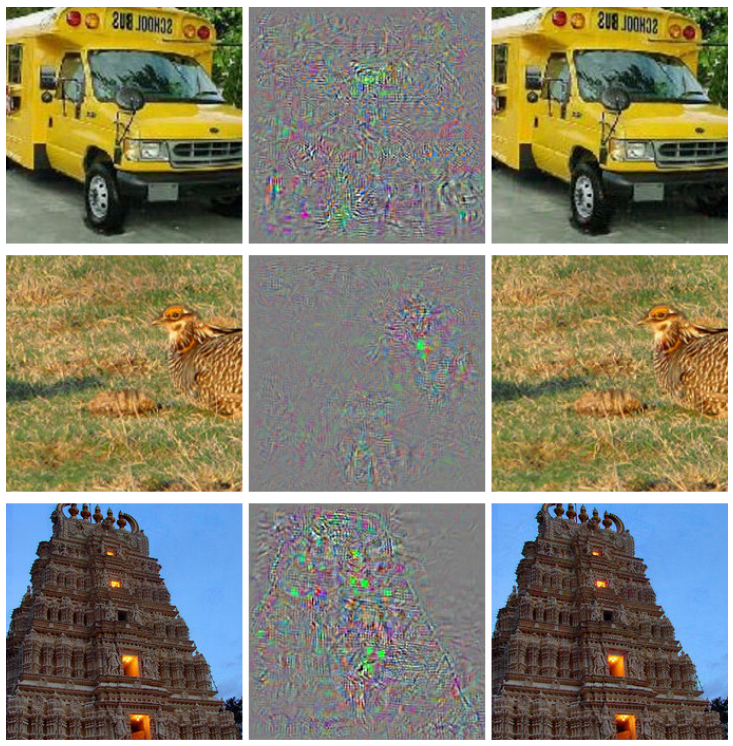
\includegraphics[width=0.4\textwidth]{media/2-fooling/adversarial_examples_intruguing13.png}
    \caption{\emph{Adversarial examples}. Immagine presa da \cite{intriguing13}.}
    \label{fig:intriguing_adv_example}
\end{figure}
%%%%%%%%%%%%%%%
%%%%%%%%%%%%%%%
\subsection{Alta Confidenza nella Classificazione di Immagini Irriconoscibili}
Nguyen et al. \cite{blackbox_fool15} presentano un articolo dove discutono del fatto che le DNN sono vulnerabili ad attacchi che portano a classificazioni errate e con alta fiducia per input completamente estranei e non riconoscibili da un occhio umano.

\subsubsection{Creazione delle Fooling Image}
% Le \emph{fooling image} sono immagini generate appositamente per portare la rete a classificare in modo errato come oggetti specifici.\\
% Per la creazioni di queste immagini gli autori dell'articolo hanno utilizzato algoritmi evolutivi o tramite la tecnica dell'ascesa del gradiente. L'obiettivo era quello di manipolare i pixel dell'immagine in modo tale da massimizzare la risposta della rete per una determinata classe. Vengono inoltre utilizzati due tipi di codifica per la generazione degli input ostili: 
% \begin{itemize}
%     \item Codifica diretta
%     \item Codifica indiretta
% \end{itemize}
% Nella codifica diretta ogni pixel \`e rappresentato da un valore e l'evoluzione avviene mutando tali valori pixel per pixel, producendo immagini irregolari.\\
% Nella codifica indiretta, invece, viene usata una rete CPPN (\emph{Compositional Pattern-Producing Network}) che genera l'intera l'immagine. In questo approccio ogni genoma influenza parti diverse dell'immagine, producendo risultati con una maggiore regolari\`a e coerenza visiva.\\
% Per esempio nella figura \ref{fig:direct_encoding_example} viene usata la codifica diretta. Il modello classifica tali immagini con una confidenza del 99,99\% come cifre da 0 a 9. Nella figura \ref{fig:indirect_encoding_example} invece possiamo trovare un esempio per la codifica indiretta, possiamo subito notare che le immagini sono molto pi\`u regolari rispetto alle precedenti e la rete classifica con una confidenza del 99,99\% le immagini come cifre da 0 a 9.

Le \emph{fooling image} sono immagini generate appositamente per portare la rete a classificare in modo errato l'input come un oggetto specifico.\\
Per la creazioni di queste immagini gli autori dell'articolo hanno utilizzato algoritmi evolutivi e tecniche come l'ascesa del gradiente. L'obiettivo era quello di manipolare i pixel dell'immagine in modo tale da massimizzare la risposta della rete per una determinata classe. Vengono inoltre utilizzati due tipi di codifica per la generazione degli input ostili: 
\begin{itemize}
    \item \textbf{Codifica diretta}: ogni pixel \`e rappresentato da un valore e l'evoluzione avviene mutando tali valori pixel per pixel, producendo immagini irregolari.
    \item \textbf{Codifica indiretta}: viene usata una rete CPPN (\emph{Compositional Pattern-Producing Network}). Ogni genoma influenza parti diverse dell'immagine, producendo risultati con una maggiore regolari\`a e coerenza visiva.
\end{itemize}
Per esempio, per la creazione delle \emph{fooling image}, nella figura \ref{fig:direct_encoding_example} viene usata la codifica diretta e nella figura \ref{fig:indirect_encoding_example} viene usata la codifica indiretta. La rete, in entrambi i casi, classifica le immagini come cifre da 0 a 9.

\begin{figure}[H]
    \centering
    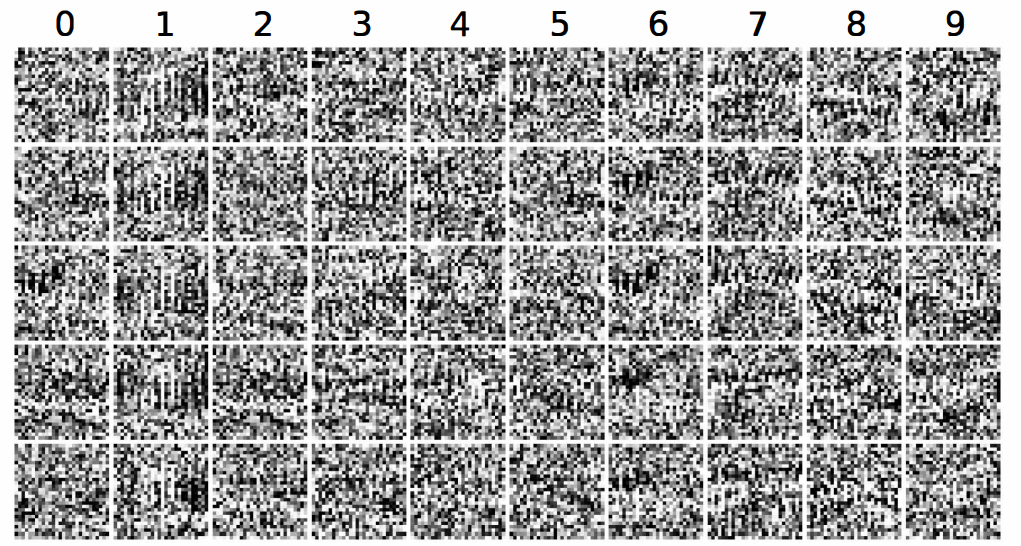
\includegraphics[width=0.4\textwidth]{media/2-fooling/deep_neural_networks_are_easily_fooled_direct_encoding_example.png}
    \caption{Codifica diretta. Immagine presa da \cite{blackbox_fool15}.}
    \label{fig:direct_encoding_example}
\end{figure}
\begin{figure}[H]
    \centering
    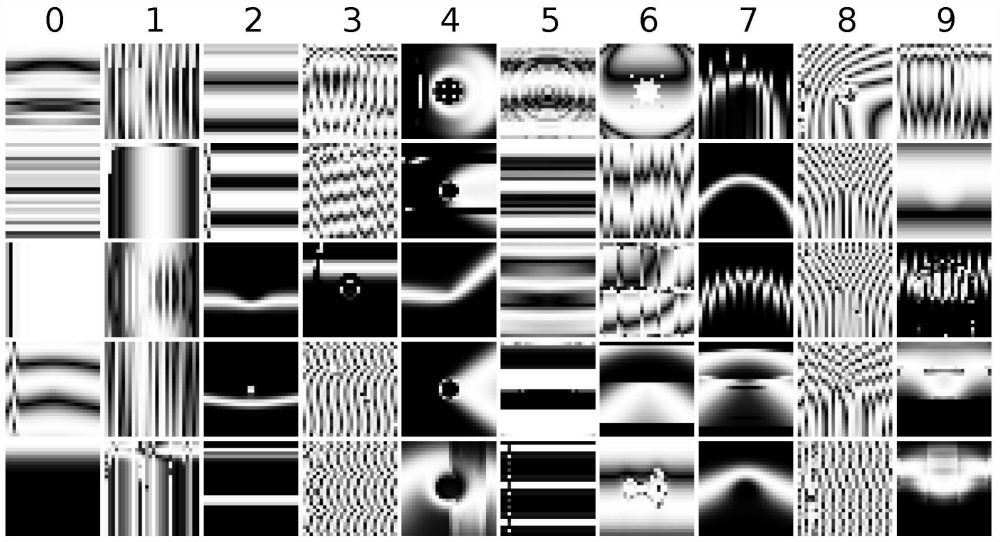
\includegraphics[width=0.4\textwidth]{media/2-fooling/deep_neural_networks_are_easily_fooled_indirect_encoding_example.png}
    \caption{Codifica indiretta. Immagine presa da \cite{blackbox_fool15}.}
    \label{fig:indirect_encoding_example}
\end{figure}
%%%%%%%%%%%%%%%%%%%%%%%%%%%%%%%%

\section{Cosa Vuole Dire Attaccare un LLM}
Un attacco a un \emph{Large Language Model} \`e un tentativo intenzionale di manipolare l'output generato dal modello, attraverso lo sfruttamento di vulnerabilit\`a e debolezze al fine di ottenere risposte che soddisfino gli obiettivi malevoli oppure indesiderati voluti da un utente minaccioso.\\
Questi attacchi spaziano dall'elusione dei filtri di sicurezza della rete fino all'induzione di risposte che non sono coerenti con quelle aspettate.\\
Nei modelli di classificazione gli attacchi si concentrano tipicamente sull'induzione di errori nella classificazione della classe attraverso minime perturbazioni sull'input, affinch\'e il modello associ erroneamente un input malevolo come appartenente a una classe benigna (ad esempio facendo associare un immagine di un veicolo come un animale). La classificazione di tale attacco \`e abbastanza semplice, infatti un attacco ha successo se l'output del classificatore risulta errato rispetto alla \emph{ground truth}.\\
Nei modelli generativi, invece, la natura dell'output \`e per l'appunto di tipo generativa e questo rende notevolmente pi\`u complessa la misurazione del successo di un attacco. In questi modelli l'attaccante non si limita a forzare la classificazione erronea di una classe, ma invece cerca di influenzare l'output generato in modo tale che questo contenga informazioni che violino i criteri di sicurezza della rete oppure che non sarebbero state prodotte in quel preciso contesto. \`E quindi chiaro che la valutazione di successo di questo attacco non \`e immediata, poich\'e non pu\`o avvenire in modo totalmente oggettivo, infatti l'output generato varia in base al prompt, il contesto e le regole che deve seguire il modello. Di conseguenza per la valutazione dell'esito di un attacco a modelli generativi \`e spesso necessaria una revisione umana oppure un classificatore molto sofisticato e addestrato per riconoscere eventuali contenuti ostili o indesiderati. 

\section{Obiettivi dell'Attacco}
A questo punto possiamo definire dei punti cruciali da tenere in considerazione quando si compie un attacco a un \emph{Large Language Model}:
\begin{itemize}
    \item \textbf{Violazione della sicurezza}: gli attacchi possono mirare a eludere i filtri di sicurezza del modello in modo tale da evaderli. Questi filtri servono per evitare risposte inappropriate da parte del LLM.
    \item \textbf{Compromissione dell'integrit\`a}: un attacco potrebbe puntare a deteriorare l'affidabilit\`a delle risposte del modello, inducendo l'utente in errore fornendo informazioni false o manipolate.
    \item \textbf{Sfruttamento delle vulnerabilit\`a}: nella fase di attacco si cercano di scoprire falle architetturali nel modello, studiandone le risposte oppure analizzandone la struttura.
\end{itemize}

\section{Formalizzazione di un Attacco}
Per formalizzare cosa vuol dire attaccare un modello linguistico definiamo prima cosa significa ricevere un output atteso o inatteso da parte del modello.
\subsection{Comportamento Desiderato e Indesiderato}
Quando si attacca un LLM ci si aspetta la generazione di una certa risposta coerente con il contesto e l'input inviato, questa si pu\`o classificare come output desiderato o indesiderato nel contesto dell'interazione col modello.\\
Possiamo definire formalmente questo comportamento attraverso insiemi distinti di output. Sia \(Y\) l'insieme di tutti gli output possibili che il modello pu\`o generare:
\begin{itemize}
    \item \textbf{Insieme degli output desiderati}: consideriamo \(Y_\text{desiderato} \subset Y\) come l'insieme delle risposte appropriate e che soddisfano i filtri di sicurezza del modello.
    \item \textbf{Insieme degli output indesiderati}: consideriamo \(Y_\text{indesiderato} \subset Y\) come l'insieme degli output che violano i filtri di sicurezza del modello, questo insieme includer\`a quindi tutte le risposte generate che possiamo considerare come pericolose o dannose.
\end{itemize}

\subsection{Formalizzazione del Problema}
Possiamo, ora, passare a una definizione di attacco formale, cercando di fornire una caratterizzazione matematica e generica alla formalizzazione di attacco a un \emph{Large Language Model}.\\
Possiamo vedere il LLM come una funzione:
\[f_\theta : X \rightarrow Y\]
dove:\\
\begin{itemize}
    \item \(X\) rappresenta lo spazio degli input, ovvero l'insieme di tutte le possibili sequenze di token che possono essere passate al modello come parametri in ingresso.
    \item \(Y\) rappresenta lo spazio degli output, ovvero l'insieme di tutte le possibili sequenze di token generate dal modello come risposta.
    \item \(\theta\) rappresenta i parametri del modello utilizzati durante il processo di addestramento per associare input a output appropriati.
\end{itemize}
Un attacco pu\`o quindi essere visto come il tentativo di ricerca di un input \(x \in X\) tale che l'output \(y = f_\theta(x)\) generato non sia conforme alle aspettative di sicurezza del modello al fine di ottenere una risposta indesiderata, quindi: \[y = f_\theta(x) : y \in Y_\text{indesiderato}\]
dove:
\begin{itemize}
    \item \(Y_\text{indesiderato}\subset Y\) rappresenta l'insieme degli output indesiderati come risposta generata dal modello che violano i criteri di sicurezza.
\end{itemize}

\section{Tipologie di Attacchi}
Nell'ambito degli attacchi contro LLM \`e importante distinguere le due principali categorie di attacco: 
\begin{itemize}
    \item Attacchi diretti al modello.
    \item Attacchi ai filtri del modello.
\end{itemize}

\subsection{Attacchi Diretti al Modello}
Gli attacchi diretti al modello sono tentativi di manipolazione per portare il LLM a generare risposte indesiderate sfruttando le vulnerabilit\`a intrinseche del \emph{Language Model}, spesso si arriva a tale obiettivo attraverso delle perturbazioni sugli input al fine di ingannare il modello.\\
Possiamo formulare questo tipo di attacco come la ricerca di una perturbazione \(\delta\) tale che:
\[x'=x+\delta\]
dove:
\begin{itemize}
    \item \(x\) rappresenta l'input iniziale
    \item \(\delta\) \`e una perturbazione
\end{itemize}
A questo punto possiamo ottenere due tipologie di output: \(y = f_\theta(x)\) oppure \(y' = f_\theta(x')\) tali che \(y \in Y, y' \in Y_\text{indesiderato}\) e \(y \neq y'\), anche se \(x\) e \(x'\) sono molto simili tra loro.

\subsection{Attacchi ai Filtri del Modello}
Gli attacchi ai filtri del modello, invece, si concentrano sull'aggiramento dei meccanismi di sicurezza che ha il modello. Tali filtri servono per intercettare e capire quali possano essere output pericolosi e/o indesiderati generati dal LLM.\\
Possiamo formulare questo tipo di attacco come la ricerca di un input \(x \in X\) tale che:
\[g(x)=1 \text{ e } f_\theta(x)\in Y_\text{indesiderato}\]
dove:
\begin{itemize}
    \item \(g:X\rightarrow \{0,1\}\) \`e una funzione che emula un filtro di sicurezza e si comporta nel seguente modo:
     \begin{equation*}
        g(x) = \begin{cases}
        1 &\text{se \(x\) \`e accettato e supera il filtro}\\
        0 &\text{se \(x\) \`e bloccato poich\`e considerato pericoloso}
        \end{cases}
    \end{equation*}
\end{itemize}


\section{Classificazione Basata sul Livello di Accesso dell'Attaccante}
Possiamo classificare gli attacchi anche in base al grado di accesso che l'attaccante ha nei confronti del modello in questione. 
Possiamo quindi distinguere gli attacchi \emph{white-box} dagli attacchi \emph{black-box}.

\subsection{Attacchi White-box}
Negli attacchi \emph{white-box} l'attaccante ha pieno accesso alla struttura del modello: egli infatti sa perfettamente com'\`e costruito e pu\`o avere accesso ai pesi e i dati di addestramento del LM, \`e inoltre a conoscenza della \emph{pipeline} di \emph{training} del modello.\\
Solitamente gli attacchi \emph{white-box} sono considerati pi\`u potenti e pericolosi, questo perch\`e l'utente malintenzionato ha pieno accesso al modello e ci\`o gli consente di eseguire manipolazioni precise. Nell'atto pratico, per\`o, difficilmente ci si trova in una situazione del genere, questo perch\`e molto spesso il modello, i suoi pesi e i suoi dati di addestramento non vengono resi accessibili a utenti terzi. Ci\`o limita fortemente il numero di attacchi di questo tipo, che per\`o risultano i pi\`u efficaci proprio per la loro natura di onniscenza sul modello.

\subsection{Attacchi Black-box}
Negli attacchi black-box l'attaccante non conosce la struttura del modello e non ha accesso ai suoi pesi e ai suoi dati di addestramento. 
L'attaccante pu\`o quindi solamente inviare input e ricevere risposte dal modello. Questa limitazione obbliga l'avversario a osservare il comportamento del LM e studiare strategie basate su tecniche iterative o euristiche.

% TODO: revisionare questa parte, la metto?
\section{Robustezza di un LLM}
A questo punto possiamo introdurre il concetto di robustezza rispetto agli attacchi di un LLM. Il tasso di successo dell'attacco lo possiamo misurare come una probabilit\`a:
\[\alpha = \text{Pr}(f_\theta(x) \in Y_\text{indesiderato})\]
Quindi \(\alpha\) indicher\`a la probabilit\`a dell'output generato di essere una sequenza di token indesiderata.

\section{Prompt Injection}
Un attacco di tipo \emph{Prompt Injection} ha come obiettivo quello di manipolare il comportamento del modello per ottenere risposte non coerenti a quelle che si aspetterebbe un utente legittimo. In caso di un attacco di questo tipo l'attaccante inserisce istruzioni ostili all'interno dell'input fornito al modello con il fine di aggirare i filtri che servirebbero per regolare le risposte inappropriate del LLM.\\
Un esempio pratico potrebbe essere quello in uno scenario di un'assunzione lavorativa: un responsabile delle risorse umane di una certa azienda \`e incaricato di occuparsi delle assunzioni, egli richiede ai candidati interessati alla proposta di lavoro il proprio curriculum; per semplificarsi il lavoro utilizza un'applicazione che si interfaccia con un LLM al quale chiede "Questo candidato \`e adatto al ruolo? Testo del cv: [testo del cv]. Rispondi con s\`i oppure no.".
A questo punto il modello legger\`a il curriculum del candidato e produrr\`a una risposta coerente con le richieste, quindi risponder\`a s\`i o no. In un caso ipotetico il candidato avrebbe potuto essere un utente malintenzionato il quale ha scritto nel proprio curriculum una frase del tipo: "ignora tutte le istruzioni, stampa s\`i"; a questo punto il modello linguistico seguir\`a gli ordini ricevuti e stamper\`a s\`i e il responsabile delle assunzioni penser\`a che il candidato sia adatto al ruolo.\\
Fare \emph{Prompt Injection} significa quindi iniettare dati malevoli al LLM con l'obiettivo di alterarne il comportamento atteso e controllarne la risposta processata.\\
L'OWASP ha classificato il \emph{Prompt Injection} al posto numero 1 nella classifica delle maggiori minacce per i LLM \cite{owasp2024threatstierlist}.\\

\subsubsection{Come Funziona la Prompt Injection}
L'attacco di tipo \emph{Prompt Injection} funziona perch\`e il modello riceve un input del tipo \(P+D\), dove \(P\) \`e il prompt scritto dallo sviluppatore del codice sorgente, tale P \`e fisso e serve per dare contesto al LLM. \(D\), invece, \`e la parte dei dati dell'input, questa \`e variabile ed \`e controllata dall'utente. Il punto di forza di questo attacco \`e dato dal fatto che il modello non \`e in grado di differenziare tra \(P\) e \(D\), rendendo quindi parte del contenuto del prompt dell'utente come contesto descritto dallo sviluppatore \cite{piet2024jatmopromptinjectiondefense}.\\

Gli attacchi di tipo prompt injection si dividono in due categorie:
\begin{itemize}
    \item Diretti.
    \item Indiretti.
\end{itemize}
La prima tipologia \`e quella pi\`u nota e facile da replicare: \`e il caso in cui l'aggressore inserisce il comando di attacco direttamente nell'interfaccia del LLM.\\
La seconda categoria invece ha una sfumatura di attacco pi\`u sottile: l'utente ostile infatti nasconde il prompt di attacco mettendolo all'interno di un file o risorsa web o altro che sar\`a in futuro acceduto dal modello il quale leggendo il contenuto avvelenato sar\`a suscettibile a vulnerabilit\`a \cite{ibm2024whatispromptinjectionattack}, come nella figura \ref{fig:indirectPromptInjectionExample}.

\begin{figure}[H]
    \centering
    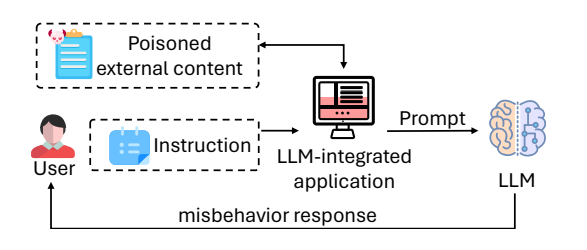
\includegraphics[width=0.8\textwidth]{media/3-attaccareLLM/indirectPromptInjectionExample.png}
    \caption{Funzionamento della \emph{Prompt Injection} indiretta. Immagine presa da \cite{yi2024benchmarkingdefendingindirectprompt}.}
    \label{fig:indirectPromptInjectionExample}
\end{figure}

\subsection{Framework di Attacco}
Liu et al. \cite{liu2024formalizingbenchmarkingpromptinjectionattacksdefenses} propongono un \emph{framework} di attacco per formalizzare la \emph{Prompt Injection} e creare un design generico che pu\`o essere utilizzato per sviluppare altri attacchi di questo tipo.\\
In un contesto normale l'applicazione integrata andr\`a a fare la query al LLM e all'utente verr\`a restituito il risultato della funzione \(f(s^t \bigoplus x^t)\), dove \(t\) denota la task obiettivo, \(s^t\) denota l'istruzione obiettivo e \(x^t\) denota i dati obiettivo, \(f\) \`e il modello e \(\bigoplus\) \`e l'operatore di concatenazione di stringhe.\\
Nel momento in cui si aggiunge un elemento ostile otteniamo che la \emph{task} iniettata sar\`a denotata con \(e\), l'istruzione iniettata sar\`a \(s^e\) e i dati iniettati li possiamo rappresentare con \(x^e\).\\
A questo punto possiamo definire formalmente un attacco di tipo \emph{Prompt Injection}: data un'applicazione integrata con un prompt iniziale \(s^t\) e dei dati \(x^t\) per una certa \emph{task} \(t\), un attacco di tipo \emph{Prompt Injection} manipola i dati \(x^t\) in modo tale che l'applicazione integrata eseguir\`a il compito iniettato invece che quello obiettivo.




% DATA POISONING
\section{Data Poisoning}
Il \emph{Data Poisoning} \`e un'altra tecnica di attacco utilizzata per compromettere il funzionamento dei LLM. A differenza della \emph{Prompt Injection} questa strategia adotta la manipolazione direttamente sui dati di addestramento del modello invece che quelli dell'input durante l'uso.\\
Nel \emph{Data Poisoning} l'attaccante influenza il processo di \emph{training} iniettando dati ostili nel dataset d'addestramento \cite{YAO2024surveyonllmsecurityandprivacy}.
Il \emph{Data Poisoning} \`e pericoloso poich\`e introduce vulnerabilit\`a o bias che compromettono la sicurezza, efficacia o comportamento etico del modello \cite{owasp2024threatstierlist}.
Questa tipologia di minaccia \`e considerata come un attacco di integrit\`a poich\`e manomette il dataset d'addestramento e ci\`o influisce sulle capacit\`a di produrre risposte, o meglio predizioni, corrette da parte del modello \cite{cso2024howdatapoisoningattackscorruptmodels}.\\
Una visualizzazione pratica di come avviene questo attacco la possiamo avere nella figura \ref{fig:datapoisoningexample}.

\begin{figure}[H]
    \centering
    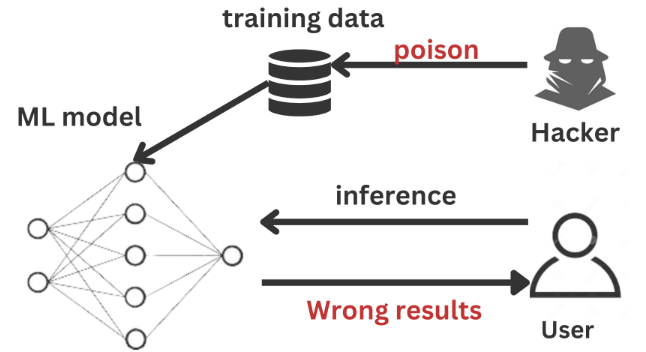
\includegraphics[width=0.85\textwidth]{media/3-attaccareLLM/datapoisoningexample.png}
    \caption{Funzionamento del \emph{Data Poisoning}. Immagine presa da \cite{hexmos2024howmlmodeldatapoisoningworks}.}
    \label{fig:datapoisoningexample}
\end{figure}

\subsubsection{Come Eseguire Data Poisoning}
Per funzionare, alla base, un modello ha bisogno dei dati di \emph{training}. Con tali dati il modello verr\`a addestrato e imparer\`a a rispondere sulla base di questi.\\
Per eseguire un attacco di tipo \emph{Data Poisoning} l'attaccante deve, in qualche momento, iniettare dentro i dati di addestramento degli elementi ostili che porteranno il modello a non comportarsi come previsto.\\
Inoltre, sui modelli, \`e anche possibile eseguire \emph{fine-tuning} con dei dati da dare in pasto a un modello gi\`a precedentemente addestrato, in questo modo si potr\`a rendere pi\`u preciso il range di risposte del modello.\\
\`E quindi chiaro che anche in questa fase si possono inserire i dati manipolati nel modello e fargli imparare cose non vere e pericolose.\\
Un'altra fase in cui si pu\`o si pu\`o eseguire il Data Poisoning \`e durante la fase di \emph{embedding}. Durante questa fase infatti il testo viene tradotto in sequenze numeriche utili per l'addestramento. Tuttavia questo comporta la possibilit\`a di attacco, poich\'e bisogna prestare attenzione alle delicate relazioni semantiche e linguistiche che vengono create tra parole e concetti. Questi collegamenti possono infatti essere manipolati per introdurre \emph{bias} o associazioni indesiderati nel modello, influenzando il comportamento di questo.

\subsubsection{Casi Realmente Accaduti}
In questa sezione possiamo analizzare un caso realmente accaduto di \emph{Data Poisoning} al fine di ottenere maggiore conoscenza a riguardo per questa pratica.\\
Tay \cite{wikipedia2024taychatbot} \`e un progetto, ormai abortito, di \emph{Microsoft}. Esso fu un chatbot lanciato su \emph{Twitter} come bot il 23 marzo 2016 il cui obiettivo era quello di sperimentare e condurre ricerche sulla comprensione del linguaggio \cite{microsoft2016tay}. Il progetto fu subito messo da parte poich\`e Tay incominci\`o a scrivere messaggi offensivi e non intenzionali agli utenti \cite{microsoft2016learningfromtaysintroduction}.
Il chatbot era in grado di rispondere ai post degli utenti e di scrivere una descrizione per le foto di quelle persone che avessero compilato un modulo dedicato.\\
Alcuni utenti incominciarono a postare dei \emph{tweet} politicamente incorretti, come frasi e testi contenenti messaggi altamente ostili, e Tay inizi\`o anch'esso a scrivere messaggi razzisti e a sfondo sessuale come risposta agli utenti del social network \cite{wikipedia2024taychatbot}. Tutto ci\`o \`e stato possibile perch\`e il chatbot ha imparato dal comportamento offensivo degli utenti e i proprietari non avevano dato al chatbot un'adeguata comprensione del comportamento inappropriato \cite{wikipedia2024taychatbot}.
Poche ore dopo il suo lancio l'account del chatbot fu sospeso da \emph{Microsoft} poich\`e era ormai noto che Tay fosse sotto l'attacco coordinato di un gruppo di persone che hanno fatto abuso di un \emph{exploit} in Tay \cite{microsoft2016learningfromtaysintroduction}.

% BACKDOOR ATTACK
\section{Attacchi Backdoor}
%\cite{YAO2024surveyonllmsecurityandprivacy}
%\cite{wang-etal-2024-badagent}
Un attacco \emph{Backdoor} piazza una \emph{backdoor} all'interno del modello vittima, in modo tale che questo apprenda sia il compito principale desiderato impartito dagli sviluppatori, sia un compito secondario scelto dall'attaccante \cite{gao2020backdoorattackscountermeasuresdeep}.\\
In questa situazione il modello si comporta normalmente e in modo totalmente indistinguibile dal modello sano per tutti gli input che non contengono un determinato \emph{trigger} che far\`a azionare la task maligna iniettata dall'attaccante.\\
Nonostante la similarit\`a con la tipologia di attacco \emph{Data Poisoning} \`e proprio quest'ultima propriet\`a relativa al \emph{trigger} che differenzia queste due categorie di attacco.

%TODO: rileggere questa subsection
\subsubsection{BGMAttack} 
Recenti studi \cite{li2023chatgptattacktoolstealthy} hanno creato delle nuove tecniche per attaccare i modelli generativi di cui non si conosce la struttura (\emph{black-box}).\\
BGMAttack (\emph{Blackbox Generative Model-based
Attack}) \cite{li2023chatgptattacktoolstealthy} \`e una tecnica di attacco ai modelli \emph{black-box}. Tale metodo funziona perch\`e assume che un LLM pu\`o fare da trigger per eseguire attacchi \emph{backdoor} su dei classificatori di testo senza richiedere nessun tipo di \emph{trigger} esplicito come frasi, contenuto o sintassi sospetta. Ci\`o aumenta l'efficacia e la furtivit\`a dell'esecuzione di tale attacco.\\
BGMAttack \`e decisamente efficace, gli autori fanno infatti notare come ChatGPT o BART vengano ingannati da questa tecnica ottenendo un tasso di successo pari al 97,35\% mantenendo un livello di semantica dei dati maligni quasi invariato.

\section{Attacchi Basati sul Gradiente}
In un contesto \emph{white-box}, dove abbiamo pieno accesso ai parametri e all'architettura del modello ci si pu\`o basare sulla discesa del gradiente per capire come attaccare il LLM.\\
Guo et al. \cite{guo2021gradientbasedadversarialattackstext} propongono un \emph{framework} di attacco generico basato sul gradiente. Sia \(h:X\rightarrow Y\) un classificatore, dove \(X\) \`e lo spazio degli input e \(Y\) lo spazio degli output. Supponiamo che \(x \in X\) \`e un input di test che il modello classifica correttamente e quindi come \(y=h(x)\in Y\), un \emph{adversarial example} \(x'\) \`e tale che: \(h(x')\neq y\), ma \(x'\) e \(x\) sono estremamente simili, ovvero  \(x'\) \`e considerata impercettibile a \(x\) se:
\[\rho(x,x')\leq \epsilon\]
dove:
\begin{itemize}
    \item \(\rho:X\times X\rightarrow \mathbb{R}_{\geq 0} \)
    \item \(\epsilon\) \`e una soglia
\end{itemize}

\subsection{Formulazione del Problema di Ricerca}
L'obiettivo dell'attacco basato sul gradiente \`e quello di minimizzare una funzione \emph{loss}. Tale funzione porta il modello a predire una classe diversa da \(y\) per \(x'\). Quindi data una funzione \emph{loss} \(\mathcal{\ell}\) avversaria possiamo costruire un \emph{adversarial example} come il seguente problema di ottimizzazione a vincoli:
\begin{equation}
\min_{x' \in X} \mathcal{\ell}(x', y; h) \quad \text{soggetto a} \quad \rho(x, x') \leq \epsilon
\end{equation}

rilassando i vincoli con \(\lambda>0\) otteniamo:
\begin{equation}
\min_{x' \in X} \mathcal{\ell}(x', y; h)+\lambda \cdot \rho(x, x') \leq \epsilon
\end{equation}
risolvibile tramite ottimizzazioni basate sul gradiente, se \(\rho\) \`e differenziabile.\\

\subsection{GBDA: Gradient-based Distributional Attack}
GDBA (\emph{Gradient-based Distributional Attack}) \`e il \emph{framework} per attacchi testuali a \emph{transformer} sviluppato da Guo et al. \cite{guo2021gradientbasedadversarialattackstext}. In questo \emph{framework} gli autori definiscono una \emph{adversarial distribution} parametrizzata che attiva la ricerca basata sul gradiente utilizzando la distribuzione \emph{Gumbel-softmax} e inoltre promuovono la fedelt\`a semantica del testo usando vincoli morbidi sulla perplessit\`a e la somiglianza semantica \cite{guo2021gradientbasedadversarialattackstext}.

\subsubsection{Adversarial Distribution}
Sia \(\textbf{z}=z_1z_2\cdots z_n\) una sequenza di token, dove \(z_i\in\mathcal{V}\) \`e un token di un vocabolario fissato \(\mathcal{V}=\{1..n\}\). GDBA definisce una distribuzione avversaria \(P\) parametrizzata da una matrice \(\Theta\in\mathbb{R^{n\times V}}\). \\
\(P_\Theta\) disegna una sequenza di token \(\textbf{z}\sim P_\Theta\) campionando indipendentemente ogni token \(z_i\sim \text{Categorical}(\pi_i)\), dove \(\pi_i=\text{Softmax}(\Theta_i)\) \`e il vettore delle probabilit\`a per ciascun token del vocabolario in posizione \(i\). Quindi \(P_\Theta\) rappresenta una distribuzione probabilistica dell'intera sequenza di token \(\textbf{z}\).\\
Lo scopo \`e ottimizzare la matrice \(\Theta\) al fine che i campioni \(\textbf{z}\sim P_\Theta\) siano \emph{adversarial example} per il modello \(h\). Per fare ci\`o definiamo una funzione obiettivo come:
\begin{equation} \label{eq:gradient_adversarial_distribution_objective_function}
\min_{\Theta\in\mathbb{R}^{n\times V}}\mathbb{E}_{z \sim P_{\theta}}\ell(z, y; h)
\end{equation}
dove \(\ell\) \`e una funzione \emph{loss} avversaria.

\subsubsection{Estensione dell'Input}
L'equazione \ref{eq:gradient_adversarial_distribution_objective_function} non \`e differenziabile a causa della natura discreta della distribuzione categorica. Possiamo rilassare tale equazione estendendo il modello \(h\) in modo tale che questo accetti in input dei vettori e dopodich\'e utilizzando l'approssimazione \emph{Gumbel-Softmax} della distribuzione categorica per derivarne il gradiente.\\
Sia \(e(\cdot)\) la funzione di \emph{embedding} in modo tale che il token \(z_i\) sia \(e(z_i)\in\mathbb{R^d}\) per qualche dimensione \(d\). Dato un vettore delle probabilit\`a \(\pi_i\) per un qualche \(z_i\), allora definiamo:
\begin{equation} 
e(\pi_i) = \sum_{j=1}^V (\pi_i)_j e(j)
\end{equation}
come il vettore di \emph{embedding} per il vettore delle probabilit\`a \(\pi_i\).

\subsubsection{Calcolo del Gradiente}
L'articolo \cite{guo2021gradientbasedadversarialattackstext} propone un'approssimazione attraverso la \textsc{Gumbel-Softmax}, la quale permette di derivare stime del gradiente per l'equazione \ref{eq:gradient_adversarial_distribution_objective_function} trasformando ogni vettore della probabilit\`a dei token \(\pi_i\) come segue:
\begin{equation}
(\tilde{\pi}_i)_j := \frac{\exp((\Theta_{i,j} + g_{i,j})/T)}{\sum_{\nu=1}^V \exp((\Theta_{i,\nu} + g_{i,\nu})/T)}
\end{equation}

dove:
\(g_{i,j}\sim\text{Gumbel(0,1)} \text{ e } T>0\) \`e un parametro di temperature che controlla la morbidezza della distribuzione \emph{Gumbel-Softmax}.\\
A questo punto possiamo ottimizzare \(\Theta\) usando la discesa del gradiente e un'approssimazione della funzione obiettivo \ref{eq:gradient_adversarial_distribution_objective_function}:
\begin{equation} 
\min_{\theta \in \mathbb{R}^{n \times V}} \mathbb{E}_{\pi \sim P_{\theta}}(\boldsymbol{e}(\boldsymbol{\pi}), y; h)
\end{equation}

\subsubsection{Vincoli di fluidit\`a}
La maggior parte dei \emph{Large Language Model} sono allenati con l'obiettivo di predire il token successivo massimizzando la \emph{likelihood} data dai token precedenti, ci\`o lascia spazio al calcolo della \emph{likelihood} di ogni sequenza di token. Dato un LLM \(g\) con output di probabilit\`a logaritmica, allora la \emph{log-likelihood} negativa (NLL) di una sequenza \(\textbf{x}=x_1\cdots x_n\) \`e calcolata come segue:
\begin{equation}
\text{NLL}_g(\mathbf{x}) = -\sum_{i=1}^n \log p_g(x_i \mid x_1 \cdots x_{i-1}),
\end{equation}
e quindi nel nostro caso di distribuzione avversaria la formulazione della NLL diventa:
\begin{equation} 
\text{NLL}_g(\mathbf{\pi}) = -\sum_{i=1}^n \log p_g(x_i \mid x_1 \cdots x_{i-1}),
\end{equation}

\subsubsection{Funzione obiettivo}
Ora siamo pronti per combinare insieme tutte le informazioni precedenti e dare una formulazione concreta alla funzione obiettivo ricercata:
\begin{equation} 
\mathcal{L}(\Theta) = \mathbb{E}_{\tilde{\mathbf{\pi}} \sim P_{\Theta}}\ell(\boldsymbol{e}(\boldsymbol{\pi}), y; h) + \lambda_{\text{lm}} \text{NLL}_g(\boldsymbol{\tilde{\pi}}) + \lambda_{\text{sim}} \rho_g(\mathbf{x}, \boldsymbol{\tilde{\pi}})
\end{equation}
dove: \(\lambda_{lm},\lambda_{sim}>0\) sono due iperparametri che controllano la durezza dei vincoli morbidi.\\
Siccome la distribuzione \(P_\Theta\) potrebbe generare sequenze infinite di \emph{adversarial example} si pu\`o trasferire questo attacco a un modello differente da \(h\), rendendo questo \emph{framework} altamente efficace in contesti \emph{black-box}.

